
\chapter{The Intermediate Period Gap}
\label{chap:period_gap}

\section*{Abstract}


Photometric variability due to stellar spots allows astronomers to measure the surface rotation periods of stars.
Within multiple missions' rotational period samples (e.g. \kepler, \ktoo, \ZTF), there is a distinct dearth of observations of stars rotating at intermediate periods 15 $\gtrsim P_{rot} \gtrsim$ 20 days.
This dearth of observations is known as the intermediate period gap.
The position of this gap varies with the colour of the stars.
Various mechanisms have been proposed to explain the dearth of observations from stars physically \update{``jumping"} the gap through enhanced wind-braking, to stars above and below the gap representing two populations of stars, to the gap representing a minima of probability to observe rotation rate.
The exact cause of the \update{gap} is currently unknown.
In this Chapter, we propose the hypothesis that the gap represents a sudden increase in the observed rotation period of stars through the onset of equator-fast latitudinal differential rotation.
The rotational period gap can be reproduced under this mechanism with observationally derived relations between equatorial and differential rotation evolution.

\newpage

\section{Introduction}
\label{sec:intro}

Measurement of the rotational period of samples of stars allows us to understand internal mechanisms that we otherwise would not be able to probe.
%%For example, the mass-dependent core-envelope coupling and decoupling of young stars have only recently been observed by measuring the rotational period of stars with age through the rotational period distribution of clusters \citep{reinhold_rotation_2015-1}.
%An unexplained feature of the rotational period distribution of low-mass main-sequence stars comes in the form of what is known as the intermediate period gap.
The intermediate period gap represents a minimum of observations of stars with particular rotation periods dependent on temperature, first observed by \citet{mcquillan_rotation_2014}.
The gap is robust between different photometric observation missions \citep{mcquillan_rotation_2014,davenport_rotating_2017,davenport_rotating_2018,lu_bridging_2022} and multiple period detection methods.
Further, the position of the gap varies in period with respect to mass. 
The quality cuts made to data sets in which rotation period is attempted to be measured \citep[e.g. removing binaries and subgiants][]{mcquillan_rotation_2014, claytor_tess_2023} are not biased away from detecting stars within the gap.
%If the gap aligned itself with a line of constant rotation in only one mission, then the mechanism underlying the gap could be more readily explained through the selection function of said mission.
These factors suggest that the intermediate period gap represents a function of stellar evolution or an unaccounted-for problem in observing rotation periods through photometric oscillations from stellar spots.

%leading the reader.
The intermediate period gap is charactertised by a number of features as shown in Figure \ref{fig:prawn}.
The density of stars above and below the gap is roughly constant; the density of observations drops swiftly.
The gap also aligns itself roughly with a line of constant Rossby number, suggesting a common phase evolution rather than age.
This is interesting because photometric variability drops toward the gap from below and above, suggesting a common phase of magnetic evolution.
We also observe that the dearth is most apparent for lower mass (\teff\ $>\ 4500K $) stars.
While, not shown in this plot, but are nonetheless indicative of the nature of the gap: the intermediate period gap disappears for fully convective stars \citep{lu_bridging_2022}.
Stars above and below the gap are also not significantly observationally distinct except in rotational period.
Further, \citet{lu_bridging_2022} argued that stars above and below the gap are of similar kinematic age.
An explanation for the gap must explain all of these features.

Multiple mechanisms have been proposed to explain the intermediate period gap.
\citet{mcquillan_rotation_2014} first proposed that the gap represents bimodal bursty star formation in the local \kepler{} field.
They suggest that the lower rotation period (faster rotators) prong represents a younger population, and the upper rotation period prong represents an older population, with the gap representing a minima in star formation at a particular time.
\citet{davenport_rotating_2018} support local bursty star formation hypothesis by separating the \kepler{} rotation period distribution by distance through \gaia{} \ parallaxes.
They find that the gap appears to disappear for stars further away than 525 pc.
At those distances, observations of stars are magnitude-limited to brighter high-mass stars (M $\geq$ 0.9 M$_{\odot}$) where observations of the gap are tentative and period detection is much less precise.
If the gap extends up to these high-mass stars, then its existence can be blurred out by the imprecision of these measurements.
Their work may also support this explanation.
In the full \citep{mcquillan_rotation_2014} sample the gap disappears for high mass ($M \ \geq \ 0.8 M_{\odot}$, $B_P - R_P \ \leq \ 1.0$) stars.
In the distance limited ($\leq$ 525pc) sample, the gap appears to permeate to these higher-mass stars. 
This can be seen in the rotational period-colour distribution in the top two panels in Figure 2 of \citet{davenport_rotating_2018} where distance is limited to 525pc.

More recent works significantly disfavour the bursty star formation hypothesis.
\citet{gordon_stellar_2021} detected the gap in multiple pointings of the \ktoo \ mission. 
In contrast, \citet{curtis_when_2020} found that the open cluster Ruprecht 147 contains stars above and below the gap, and a possible star detection within the intermediate period gap.
This suggests that the gap is not a coeval feature and instead a feature of the rotational evolution of low-mass stars.
\citet{curtis_when_2020} instead proposed that the gap aligns with a line of constant Rossby number ($R_o\sim 0.6$), rotation rate scaled quantity shown to be associated with the magnetic activity of stars.

As of writing, there are two leading explanations for the gap.
First, consider that the intermediate rotational period gap represents a sudden onset of extreme rotational braking.
\citet{mcquillan_rotation_2014} suggested another explanation for the intermediate period gap through a rapid spin-down - ``jumping" across the gap quickly, resulting in decreased stars' density in this period-colour space region.
For example, the rapid spin-down could be caused by core and convective envelope rotational decoupling at the upper edge of the lower prong near the rotational period gap.
In this mechanism, the core and envelope evolve independently; the envelope, having a much smaller moment of inertia than the core, is spun down rapidly under the same magnetic braking conditions.
Following the gap, the core and envelope then recouple, exchanging angular momentum and returning to a normal rate of magnetic braking. 
\citet{gordon_stellar_2021} argued in favour of this hypothesis based on the rotation period distribution of \ktoo{} data. 
\citet{curtis_when_2020} argued that two-zone angular momentum transport models, such as those by \citet{spada_competing_2020} can reproduce a stalled braking behaviour required to explain the lower prong of the intermediate rotational period gap, but their model could not explain the rapid-spin down.
This hypothesis is generally supported by the tentative observation of low-mass fully convective stars permeating the gap as well as the observed similar ages of stars above and below the gap \citep{lu_bridging_2022}.

The other leading theory is that the gap results from a low probability of observing stars within the gap.
\citet{chahal_statistics_2022} proposes that the gap results from the low magnetic activity of stars within the gap resulting in very few expressed stellar spots and, thus, a low probability of observing stars in the gap.
\citet{reinhold_transition_2019} and \citet{reinhold_stellar_2020}, however, proposed that the gap is caused by a transition in activity from spot dominance to bright facula dominance \footnote{This work differentiates between the rotation brightness modulation and brightness modulation from the stellar activity cycle. Stellar activity modulation refers to the long-term evolution of average brightness due to stellar spots and faculae rather than variations on the rotational time scale.}.
They suggest that as a star spins down and the magnetic field topology changes, the initially strong and long-lived spots are replaced by smaller, short-lived spots surrounded by bright faculae.
In such a scenario, the photometric variability amplitude decreases because of the partial cancellation by the increase and decrease in brightness from the faculae and spots.
Hence, the stars with small photometric variability will not be detected.
These mechanisms are supported by the gap aligning with a line of constant Rossby number and by the photometric variability reaching a local minimum surrounding the gap.


%On the other hand, if the gap results from a low probability of observing stars within the gap, we have undoubtedly observed gap stars, spectroscopically or asteroseismically, that we do not know are gap stars.
%Therefore, whether gap stars are peculiar - photometrically, spectroscopically or asteroseismically - is unknown.
%Gap stars may have been previously flagged as peculiar, but the link between the gap and these stars has never been made.
%On the other hand, gap stars may not be otherwise peculiar - chemically or, say, in terms of magnetic activity.
%If indeed they are not otherwise peculiar, then, oxymoronically, the reason for their lack of observation raises more questions about the mechanism underlying the gap.

\update{If either of these theories are correct they have implications for the evolution of rotation and magnetic activity within stars.
There is, however, little evidence to confirm either of their involvement in the observation of the intermediate period gap.}
We propose a previously uninvoked mechanism to consider: the onset of latitudinal differential rotation.
Stars, most concretely for the Sun, have been observed to express latitudinal differential rotation.
Further, stars express latitudinally distributed spots across their surface.
Which raises the question: what is the ``surface rotation period'' of a star?
Radially symmetric (1D) models of rotating stellar evolution provide a measure of the ``average" surface rotation rate of stars, but then if the rotation profile varies latitudinally, what does that surface rotation rate map to?
The observed rotation rate of stars measured from stellar spots is generally taken as the average rotation rate where stellar spots are expressed \citep{santos_surface_2021}, but how well do those values map to models of stellar rotation?
The terms are ill-defined, but we intend to bridge the gap between these two facets by considering the effect that latitudinal differential rotation has on the observed rotation periods of stars.
Specifically, whether a swift transition from flat to latitudinally differentially rotating introduces significant variations to the observed rotation period, resulting in the intermediate period gap.

\update{Qualitatively, observations \citep[see, e.g.,][]{saar_starspots_2011, benomar_nearly_2015, benomar_asteroseismic_2018, bazot_latitudinal_2019, hall_weakened_2021} and magnetohydrodynamic models of stars including latitudinal differential rotation \citep[see, e.g.,][]{brun_powering_2022} suggest three regimes of latitudinal differential rotation dependent on Rossby number.
Their results suggest fast-rotating stars ($R_o < 0.45$) support quenched, latitudinally flat\footnote{Or rather, close to latitudinally flat.} rotation profiles.
In this regime, the scale of equator-fast differential rotation, defined as the absolute difference between the rotation rate at the equator and at a latitude of 60$^{\circ}$ divided by the equator rotation rate, increases with $R_o$.
The scale of differential rotation swiftly grows in this regime until it saturates, resulting in intermediate rotating stars ($0.45 \ \leq \ R_o \  \leq \ 2$) expressing constant scale equator-fast differential rotation.
As a star approaches $R_o \sim 2$ meridional transport of angular momentum from the equator to the pole is expected to slow the rotation rate near the equator \citep{amard_rotating_2016}.
This, in combination with angular momentum loss through magnetised stellar winds, is expected to result in a supposed transition from equator-fast to equator-slow latitudinal differential rotation\footnote{While this transition is theoretically expected, equator slow differential rotation has not been observationally verified.}.
The relationship between the scale of differential rotation in this regime is unknown due to a lack of observations of equator-slow differential rotation.}

Interestingly the transition from latitudinally flat rotation profiles, to equator fast rotation profiles occurs near $R_o \sim 0.5$, the Rossby number where the rotational period gap occurs.
If latitudinal differential rotation becomes significant at this point in the evolution of rotation of a star, then the rotation period gap may reflect a sudden increase in average, and thus observed, surface rotation period from that onset.
In this work, we qualitatively investigate this as a possible mechanism underlying the intermediate period gap by creating a physically motivated observed rotation period distribution under the differential rotation relationships proposed by \citet{saar_starspots_2011} and \citet{brun_powering_2022}.
In Section \ref{sec:methods}, we describe the adopted relationships between latitudinal differential rotation and Rossby number, our choices of stellar parameters, as well as our adopted method to calculate an observed rotation period.
In Section \ref{sec:results}, we present the observed rotational period distributions of the synthetic sample, compared to the observed \kepler \ rotational period distribution.
Finally, in Sections \ref{sec:discussion} and \ref{sec:conclusion}, we place those results into context by discussing the implications of our discovery, discuss the impact of the uncertain model parameters, and propose extensions to this work.


\section{Methods}
\label{sec:methods}

\update{We prepare a sample of observed rotational periods of stars with latitudinal differential rotation.
The stellar parameters we adopt in this work are physically motived but the resulting rotational distribution is intended to only be indicative of the effect that latitudinal differential rotation has on the observed rotational period distribution.}
%todo: we may need to update this depending on what we change
We generate 30,000 main-sequence and early post-main-sequence stars with various values of mass, age, metallicity and rotation rate.
We drew masses from a uniform mass function between 0.65 and 1. 
This limits our range of masses to those with a radiative surface and convective core and especially targets stars where the rotational period gap is most apparent. 
We have not assumed an initial mass function here - this is because the \kepler{} sample is biased towards brighter high-mass stars, which we assume here effectively cancels out, say, a Saltpeter IMFs bias towards a larger number of low-mass stars.

%todo:check this with Andy
Metallicity is drawn from a distribution to approximately reflect what is observed in the Milky Way. Specifically, we defined a variable $\phi$ to be drawn from a Beta distribution
\begin{equation}
  \phi \sim \mathcal{B}\left(\alpha=10, \beta=2\right)
\end{equation}
and applied a transform from $\phi$ to [Fe/H] by requiring the metallicities be bounded between $[\mathrm{Fe/H}]_\mathrm{min} =-2$ and $[\mathrm{Fe/H}]_\mathrm{max} = +0.5$. We also required that the mode of $\phi$, defined as $\frac{\alpha - 1}{\alpha + \beta - 2}$ for a Beta distribution, occurs at Solar metallicity. This leads to the transform:
\begin{equation}
  [\mathrm{Fe/H}] = \left(\frac{}{}[\mathrm{Fe/H}]_\mathrm{max}-[\mathrm{Fe/H}]_\mathrm{min}\right)\left(\phi - \frac{\alpha - 1}{\alpha + \beta - 2}\right) \quad .
\end{equation}

The stars we generate mock data for in this work span from the ZAMS to low-luminosity subgiants. We draw equivalent evolutionary phase values from a uniform distribution EEP $\sim \mathcal{U}(200,450)$, where $\mathcal{U}\left(a,b\right)$ denotes a uniform prior between $a$ and $b$.
The bounds of this range (200 and 450) represent the ZAMS and the low-luminosity subgiant phase, respectively. 
Using the EEP, mass and metallicity, we interpolate a position along the MIST stellar isochrones \citep{morton_isochrones_2015} to calculate the expected \teff \ and \logg \ for each star.
We also obtain the star's age (post-ZAMS) that we can use in conjunction with the other stellar parameters to determine rotational properties. 

The surface equator rotation period ($P_{\rm{surf}}$) is then interpolated from stellar cluster-tuned rotational isochrones given the stellar age and mass (Table A1 in \citet{spada_competing_2020}).
This sample does not produce the observed rotational period gap and results in a smooth density of rotational periods around the $R_o =0.5$.

We evaluate the first evaluate the convective turnover timescale ($\tau_c^{\rm{CS}}$) of our sample using the scaling relation derived in \citet{cranmer_testing_2011},
\begin{equation}
	\tau_c^{\rm{CS}} = 314.24 \ \exp\left[ -\frac{T_{\rm{eff}}}{1952.5\rm{K}} - \left( \frac{T_{\rm{eff}}}{6250 \rm{K}}\right)^{18}\right] + 0.002 d
\end{equation}
from this we calculate $R_o$ of our sample ($R_o = P_{\rm{surf}}/\tau_c^{\rm{CS}}$).

The scale and sign of differential rotation varies with $R_o$.
We adopt the 3 different piecewise functions to represent the evolution of the scale of differential rotation between the equator and at a latitude of 60$^{\circ}$.
The first is the observational trend described in \citet{saar_starspots_2011}, where the scale of differential rotation grows with $R_o^{2.5}$ while $R_o \ \leq \ 0.45$ and is constant above this limit,
\begin{equation}
\label{eq:rot_ex}
{\centering
\frac{|\Delta\Omega|}{\Omega_{\rm{s}}} = \left\{
\begin{array}{ll}
   0.2/(0.45^{2.5}) R_o^{2.5}& R_o\leq 0.45 \\
   0.2 & 0.45 \leq R_o
\end{array} 
\right.}
\end{equation}
where we have ensured continuity with the prefactor $0.2 \ / 0.45^{2.5}$, and $\Delta \Omega$ is the difference between the equator rotation rate and the rotation rate at a latitude of 60$^{\circ}$ and $\Omega_{\rm{surf}}$ is the average surface rotation rate.

The other two relations we adopt reflect two cases for the transition of the scale of differential rotation that are steeper than the \citet{saar_starspots_2011} relation that fall within the range suggested by the edges of the scale of differential rotation in \citet{brun_powering_2022} (See Figure 8 in their work).
These relations are:
\begin{equation}
{\centering
\frac{|\Delta\Omega|}{\Omega_{\rm{s}}} = \left\{
\begin{array}{ll}
   0.2/(0.45^4) R_o^4& R_o\leq 0.45 \\
   0.2 & 0.45\leq R_o\leq 2 \\
   0.2/(2^2) R_o^2& 2\leq R_o \\
\end{array} 
\right.}
\end{equation}

and

\begin{equation}
{\centering
\frac{|\Delta\Omega|}{\Omega_{\rm{s}}} =  \left\{
\begin{array}{ll}
   0.2/(0.45^6) R_o^6& R_o\leq 0.45 \\
   0.2 & 0.45\leq R_o\leq 2 \\
   0.2/(2^2) R_o^2 & 2\leq R_o \\
\end{array} 
\right.}
\end{equation}
where the prefactors $0.2 \ / \ 0.45^{4}$, $0.2 \ / \ 2^{4}$, $0.2 \ / \ 0.45^{6}$, and $0.2 \ / \ 2^{2}$ ensure continuity.
We have chosen these two relations to investigate the effect of the steepness of the relation between differential rotation and $R_o$ on the observed rotational period distribution as well as the effect of an increase to the scale of differential rotation beyond $R_o = 2$.
The relations we investigate in this work are shown in Figure \ref{fig:compar_diffrot}, where we show the relation determined in \citet{saar_starspots_2011} (orange), the range of the scale of differential rotation suggested by \citet{brun_powering_2022} and the two steeper relations (green and purple respectively) relations we adopt in this work.

\begin{figure}
\centering
  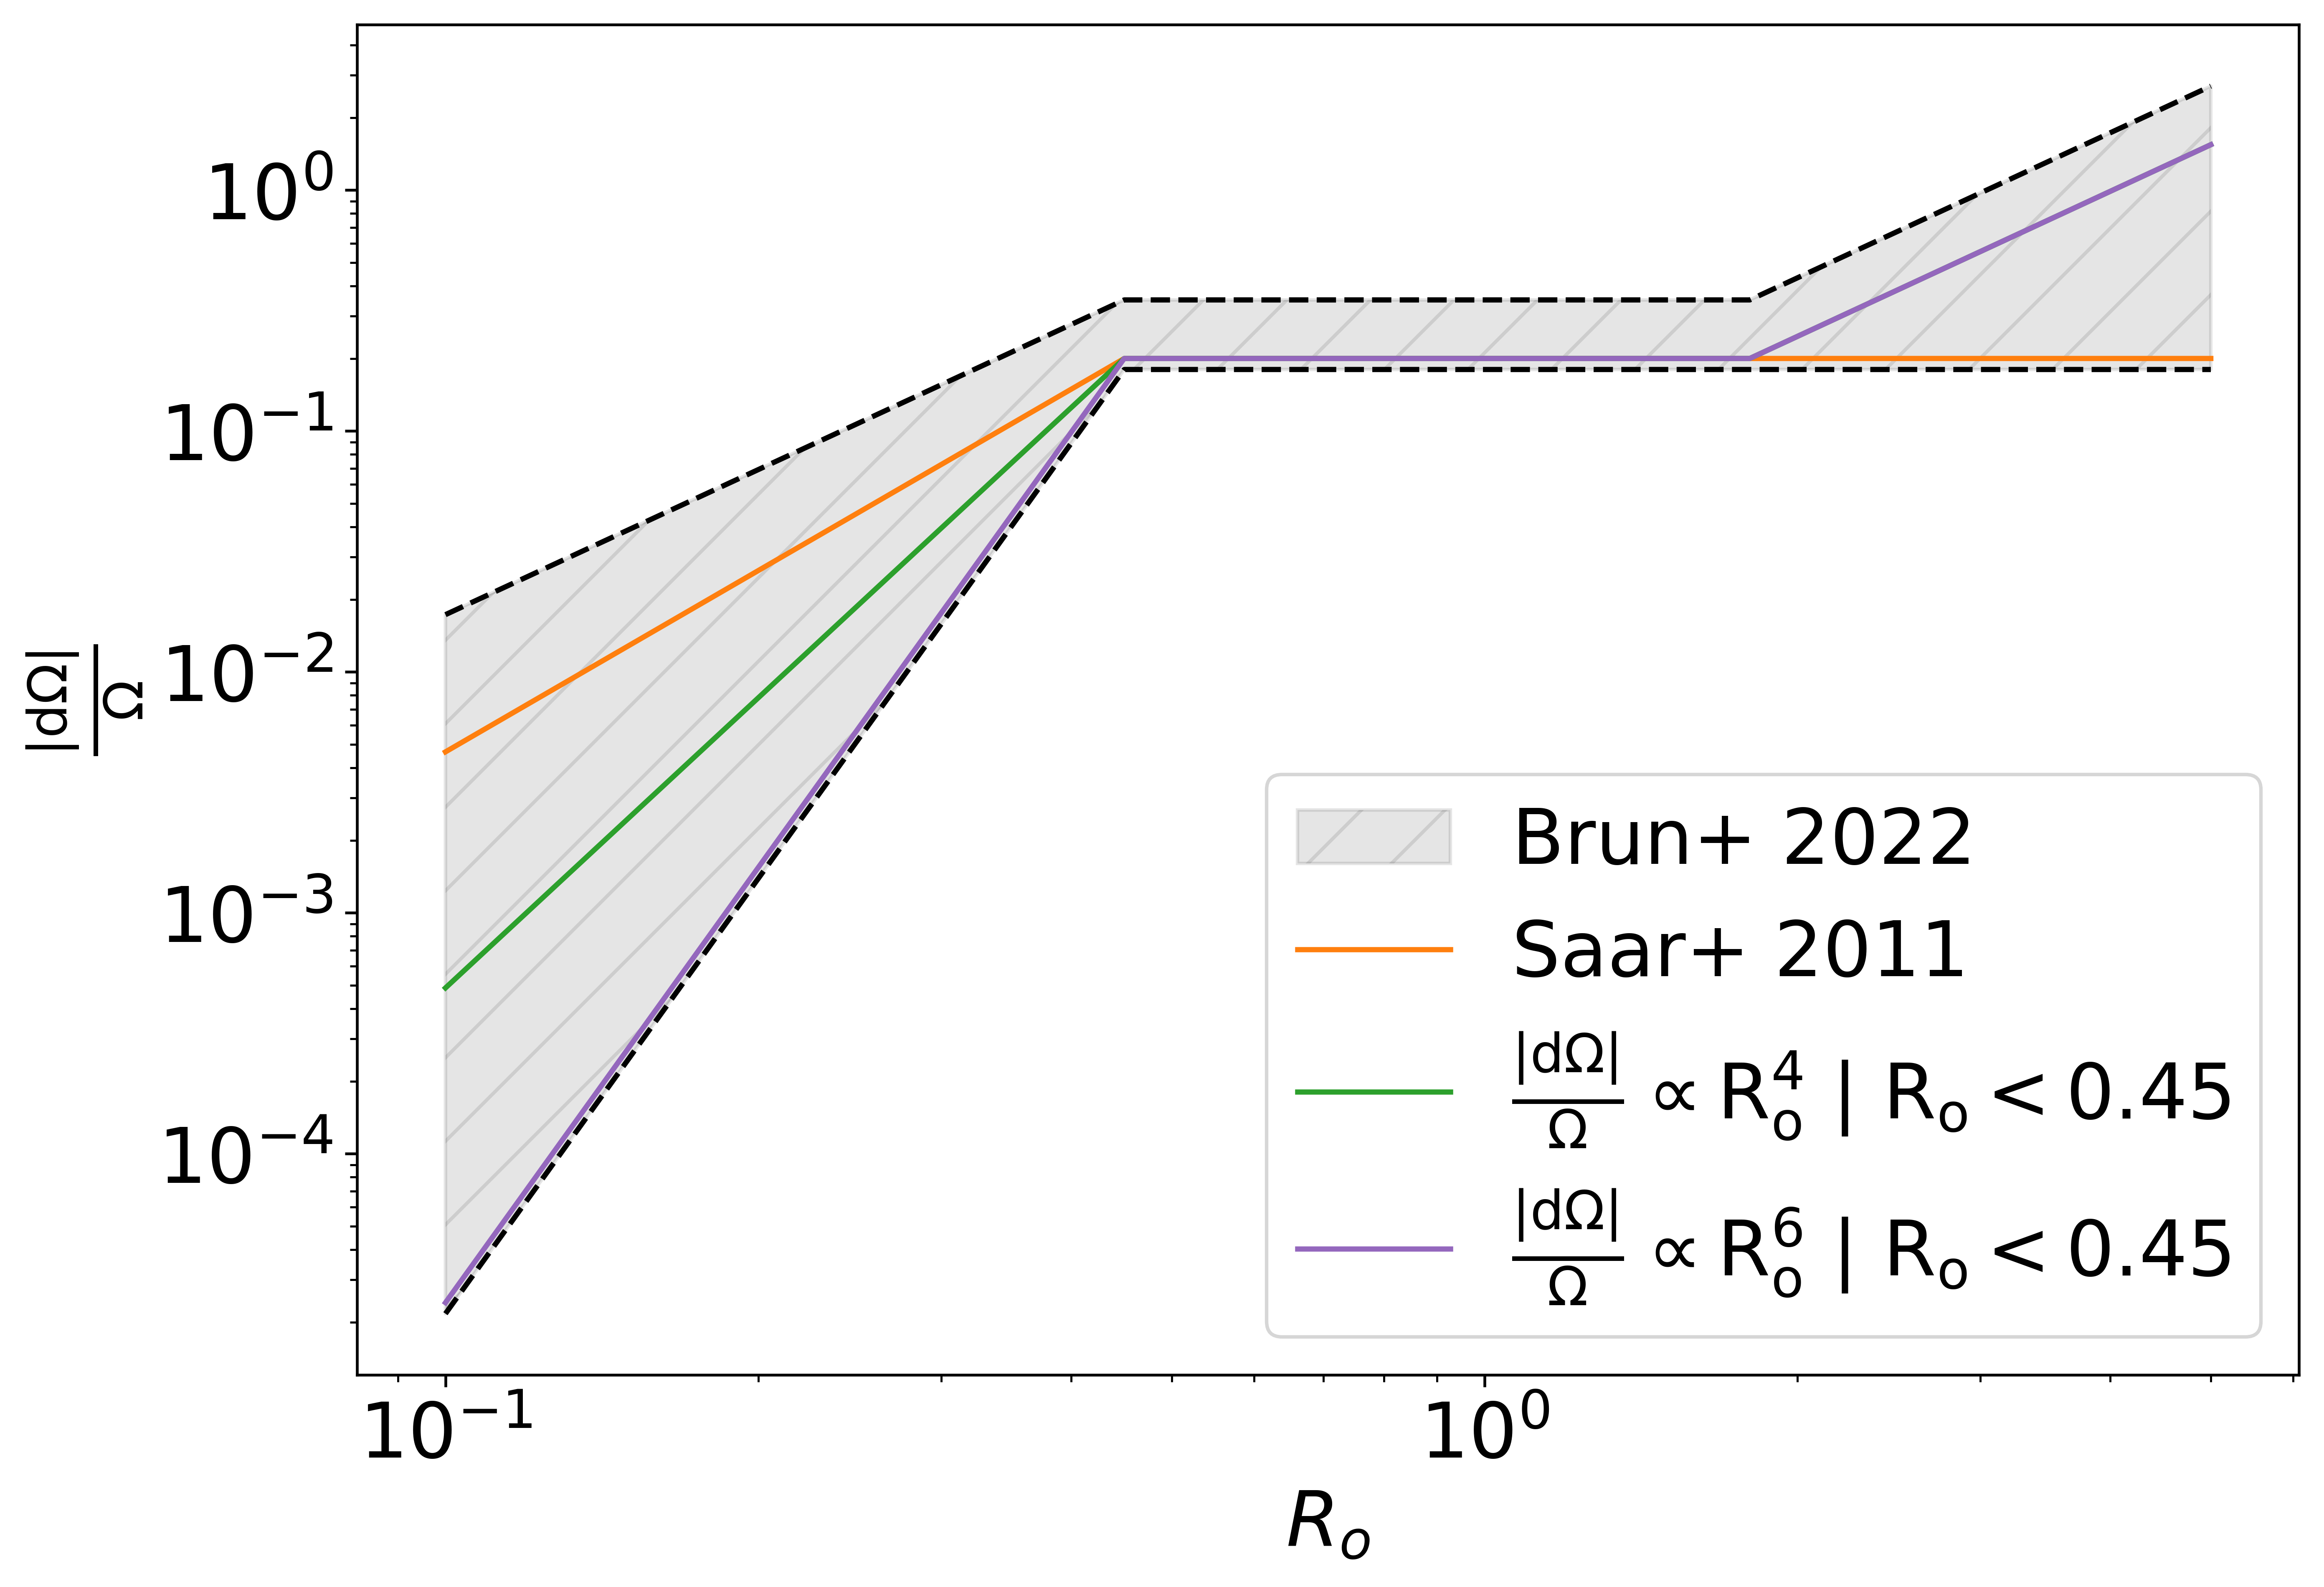
\includegraphics[width=\textwidth]{Figures/rot_gap_figures/comparison_diffrot.png}
  \caption[The various relationships between latitudinal differential rotation and the stellar $R_o$ adopted in this work.]{
  	The various relationships between latitudinal differential rotation and the stellar $R_o$ adopted in this work. We compare between the observationally derived relation from \citet{saar_starspots_2011} (orange) and two steeper relations for $R_o\leq0.45$, $|\Delta \Omega|/\Omega \propto R_o^4$ (green) and $|\Delta \Omega|/\Omega \propto R_o^6$ (purple). The scale of differential rotation is greater for the latter two relations and we have an increase to the scale of differential rotation for $R_o\geq2$. All three relations are consistent with the magnetohydrodynamic investigations into stellar differential rotation from \citet{brun_powering_2022}.
}
  \label{fig:compar_diffrot}
\end{figure}

Here we assume that for $R_o \ < \ 2$, stars express equator-fast differential rotation, therefore the sign of $\frac{\Delta \Omega}{\Omega_{\rm{s}}}$ is positive.
Above $R_o \ = \ 2$ the star instantly transitions to equator-slow, and the sign becomes negative. 
From this, we calculate the differential rotation by multiplying this factor by the equator rotation rate.
While the instantaneous nature of this transformation may not be physical, the transition from solar-like to anti-solar-like differential rotation will have the same effect: an increase in the density of stars with observed rotational periods near the transition.

We adopt a second-order solar-like differential rotation profile with the rotation rate with the spherical coordinate, $\theta$,
\begin{equation}
    \label{eq:obs_eq}
    \Omega\left(\theta\right) = \Omega_{\rm{eq}} - \frac{\Delta \Omega}{\cos^2 60^{\circ}} \sin^2{\theta}.
\end{equation}
$\theta$ is the angle measured from the pole of each latitudinal band ($\theta$ is the latitude minus $\pi/2$) and the factor $\frac{1}{\cos^2{60^{\circ}}}$ ensures that the rotation rate is $\Delta \Omega + \Omega_{\rm{eq}}$ at 60$^{\circ}$ (from the definition of $\Delta \Omega$).
This provides us with our expression for the latitudinal differential rotation profile of our stars given the equator rotation period.

We then calculate the observed rotation rate from the integral of the rotation rate given a distribution of stellar spots on a star's surface divided by the star's surface area, both calculated where the stellar spots are expressed.
Here we are assuming that all stars in our sample are viewed equator-on.
While this is not the case for all stars, the rotational period gap is not an effect of the observation angle.
Further, inclination angles are uniformly distributed in $\cos{i}$, and stars must be viewed close to equator-on for stellar spots to introduce significant variations to the light curve as a star rotates. 
Therefore, most stars with observed rotation periods are close to equator-on.

The distribution of stellar spots on the surfaces of these stars requires some thought.
The probability distribution of stellar spots on the surface of the Sun is well known \citep[see, e.g.,][]{maunder_note_1904,hathaway_solar_2015}.
While we could adopt a solar distribution this does not account for various effects.
For example, the latitudinal distribution of active regions vary along the stellar magnetic cycle \citep[see, e.g.,][ and references therein]{grijs_stellar_2021}.
Further, adopting such a distribution would not account for star-to-star such as variations with stellar mass, equator rotation rate,  and the scale of differential rotation both radially and latitudinally.
For this reason the treatment of the distribution of stellar spots is a major source of uncertainty in our work.
For now we adopt a uniform distribution of stellar spots between the latitudes of $0^{\circ}$ and $60^{\circ}$.
We will discuss the effect that this uncertainty has on the conclusions we draw in Section \ref{sec:discussion}.

If the stellar spots are uniformly distributed, then the observed rotation rate of the surface is simply the average rotation rate between the edges of the latitudes where the stellar spots are expressed.
The average rotation rate is calculated from the integral of the rotation rate divided by the surface area both over the maximum and minimum latitudes that the spots are expressed,
\begin{equation}
\label{eq:inte}
	\Omega_{\rm{obs}} = \int^{\theta_{\rm{max}}}_{\theta_{\rm{min}}} \Omega(\theta) \sin(\theta) \rm{d}\theta \ / \  \int^{\theta_{\rm{max}}}_{\theta_{\rm{min}}} \sin(\theta) \rm{d}\theta
\end{equation}
where rotation rate is independent of radius and azimuthal angle, and their contributions cancel.
Here $\theta_{\rm{max}}$ and $\theta_{\rm{min}}$ are the upper and lower bounds of the distribution of spots on the surface of the star.
Because the rotation profile is symmetric about the equator of rotation we only need to calculate the contribution to the rotation rate in one hemisphere.

We compare the effect of each of the chosen relations between differential rotation and $R_o$ on the observed rotation period of $0.7 M_{\odot}$ star in Figure \ref{fig:comp_per}.
The growth of differential rotation below $R_o <  0.45$ is observed at $P_{\rm{rot, injected}} < 20$ d.
Steeper relations of $R_o$ with differential rotation in this range result in a quicker growth in observed rotation periods for the same injected period.
The steeper the growth of the observed rotational period, the lower the number of stars that would be observed with that rotational period, while the transition from equator-fast to equator-slow differential rotation rotation ($P_{\rm{rot, injected}} \ = \ 70$ d) results in an instantaneous transition from observed rotational periods greater than the injected value, to an observed rotational period less than the injected value.

\begin{figure}
\centering
  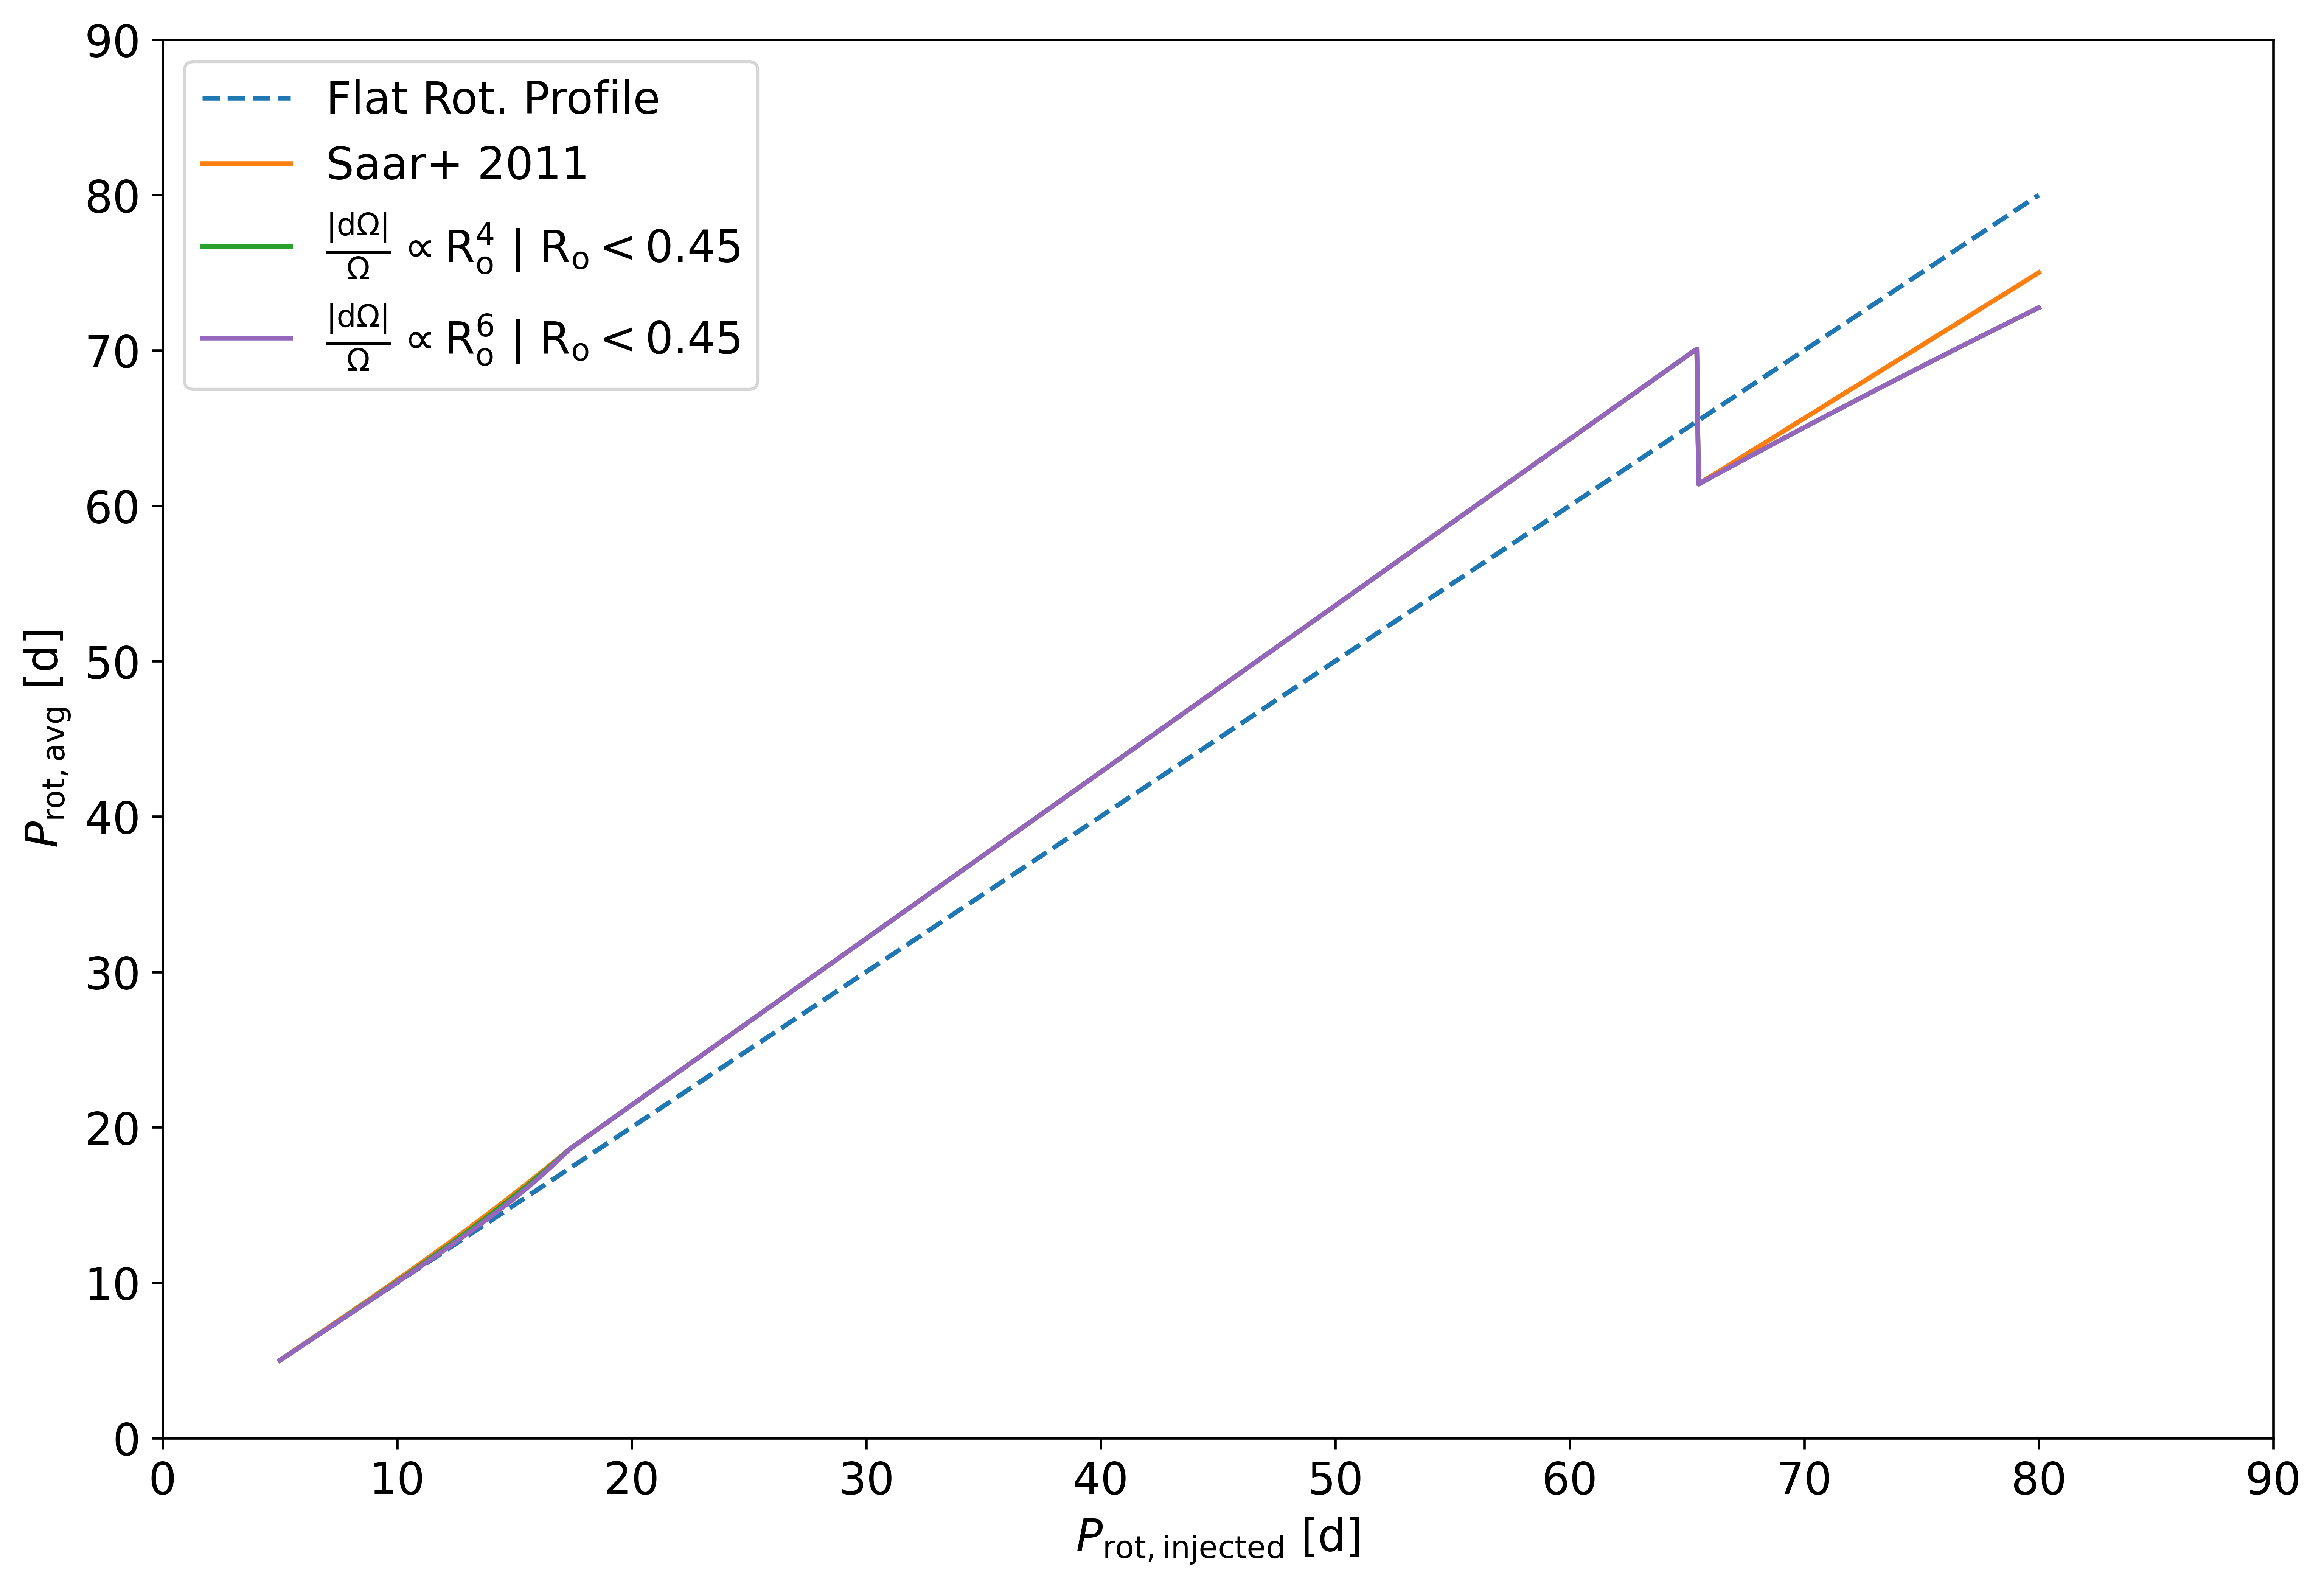
\includegraphics[width=\textwidth]{Figures/rot_gap_figures/comparison_observed_rot_periods.png}
  \caption[The effect of the differential rotation on the observed rotational period of a 0.7 $M_{\odot}$ star against $R_o$.]{
  	The effect of the differential rotation on the observed rotational period of a 0.7 $M_{\odot}$ star. Here the colour of the relations corresponds to the adopted differential rotation relation in Figure \ref{fig:compar_diffrot} compared to the observed rotation profile of a latitudinally flat rotating star. At $R_o<0.45$ for injected rotation periods ($P_{\rm{rot, injected}}$) less than 20 days. It is evident that steeper relations between $R_o$ and differential rotation lead to more rapid growth in observed rotation periods for the same injected period. Moreover, a steeper growth in the observed rotational period corresponds to a lower number of observed stars with that particular rotation period. The transition from solar-like to anti-solar-like rotation, occurring at $P_{\rm{rot, injected}}$ = 70 days, results in an instantaneous shift in observed rotational periods from being greater than the injected value to being less than the injected value.
}
  \label{fig:comp_per}
\end{figure}

\section{Results}
\label{sec:results}
The observed rotation period under each relation of differential rotation and $R_o$ of the stars in our synthetic sample can then be calculated.
The resulting distributions of stars (blue, orange, green and purple) relative to the observed distribution of \kepler{} rotational periods measured in \citet{mcquillan_rotation_2014} (black) are shown in Figure \ref{fig:comp_dist}.
Here, the colour of each distribution corresponds to the same colour showing the relation between differential rotation and $R_o$ in Figure \ref{fig:compar_diffrot} and blue corresponds to the injected, or flat rotation profile observed, rotational period.

In Figure \ref{fig:comp_hess} we show how the adopted relations impact the rotational period distributions.
In the left column we show the 2D histogram of the \citet{mcquillan_rotation_2014} rotational period distribution.
In the middle column we shown the 2D histogram of the observed rotational period distributions under the adopted relations between latitudinal differential rotation and $R_o$.
From top to bottom panel we show the injected rotational periods from our generative model (with no latitudinal differential rotation), then under the \citet{saar_starspots_2011} differential rotation relation, then with$\frac{|\Delta\Omega|}{\Omega_{\rm{s}}} \ \propto R_o^4$ model, and finally with $\frac{|\Delta\Omega|}{\Omega_{\rm{s}}} \ \propto R_o^6$.
These correspond to the blue, orange, green, and purple distributions in Figure \ref{fig:compar_diffrot} respectively.
All of the panels in the left two columns are colour by the number of stars in each bin: N$_{\rm{Obs.}}$ for the left column and N$_{\rm{Mod.}}$ for the middle.
In the right column we show the difference between the distributions through N$_{\rm{Obs.}}$ and N$_{\rm{Mod.}}$ for each adopted relation.
Darker colours correspond to regions where the model over predicts observations and lighter where the model under predicts observations.

Our models predicts a dearth of observations, coincident with the intermediate period gap as a result of the transition from latitudinally flat to equator-fast differential rotation at $R_o = 0.45$.
This can be seen comparing the top panel to the bottom three in the right column of Figure \ref{fig:comp_hess}.
Latitudinal differential rotation decreases the difference between the observed and model rotational periods.
Further, the increased density of observation of stars above the intermediate period gap in the \kepler{} sample is reproduced under this model, unlike a model of extreme magnetic braking to explain the gap.
The distinctness, or rather the decrease in density of stars within the gap, increases with the power on $R_o$ when $R_o \leq 0.45$.
We also find that our models predict an over-density of stars where the transition from equator-fast to equator-slow latitudinal differential rotation occurs ($\log P_{\rm{rot}} = 1.2$, $T_{\rm{eff}} = 6000K$).

\begin{figure}
\centering
  \includegraphics[width=\textwidth]{Figures/rot_gap_figures/comp_dist.png}
  \caption[The observed rotational period distributions of the synthetic sample of stars given various relations between latitudinal differential rotation and $R_o$ overlayed over the observed distribution of rotational periods of the \kepler{} sample from \citet{mcquillan_rotation_2014} (black).]{
  	The observed rotational period distributions of the synthetic sample of stars given various relations between latitudinal differential rotation and $R_o$ overlayed over the observed distribution of rotational periods of the \kepler{} sample from \citet{mcquillan_rotation_2014} (black). Here, the coloured observed rotational period distributions correspond to the various differential rotation relations adopted in this work, as seen in Figure \ref{fig:compar_diffrot}. The latitudinally flat (blue, top left) sample reflects the injected rotational periods of our sample considered in this work. We observe that there is no intermediate period gap in this synthetic sample of stars without differential rotation. If we include the effects of differential rotation on the observed rotation period, a dearth of observations at the transition between latitudinally flat ($R_o<0.45$) and solar-like rotation occurs precisely at the location of the intermediate period gap. 
 Further, we find that as the steepness of the relation between $|\Delta \Omega| / \Omega$ increases (where in order of increasing steepness, we have the orange, green and purple distributions) the gap becomes more distinct - fewer stars are observed within the gap. We also find that due to the transition from solar-like to anti-solar-like differential rotation, we obtain an over-density of stars consistent with the overdensity of slow-rotating stars near 6000K. See \ref{fig:comp_hess} for 2D histograms of the distribution of rotation periods in these panels.}
  \label{fig:comp_dist}
\end{figure}

\begin{figure}
\centering
  \includegraphics[width=\textwidth]{Figures/rot_gap_figures/comp_hess.png}
  \caption[2D histograms of observed and the synthetic observed rotational period distribution assuming various relations between the scale of differential rotation and $R_o$ and the difference between the two.]{
2D histograms of observed and the synthetic observed rotational period distribution assuming various relations between the scale of differential rotation and $R_o$ and the difference between the two.
\textbf{Left:} 2D histogram of the \citet{mcquillan_rotation_2014} rotational period distribution.
\textbf{Middle:} 2D histogram of the observed rotational period distributions under the adopted relations between latitudinal differential rotation and $R_o$. From top to bottom panel we show the injected rotational periods from our generative model (with no latitudinal differential rotation), then the relation under the \citet{saar_starspots_2011} differential rotation relation, then with $\frac{|\Delta\Omega|}{\Omega_{\rm{s}}}$ $\propto R_o^4$, and finally with $\frac{|\Delta\Omega|}{\Omega_{\rm{s}}}$ $\propto R_o^6$.
These distributions correspond to the blue, orange, green, and purple distributions in Figure \ref{fig:compar_diffrot} respectively.
All of the panels in the left two columns are colour by the number of stars in each bin: N$_{\rm{Obs.}}$ for the left column and N$_{\rm{Mod.}}$ for the middle.
\textbf{Right:} The difference between the distributions: N$_{\rm{Obs.}}$ - N$_{\rm{Mod.}}$ for each adopted relation.
Darker colours correspond to regions where the model over predicts observations and lighter where the model under predicts observations. We observe that the accounting for differential rotation when determining the expected observed rotation periods of stars introduces a decrease in density of observations where significant differential rotation arises (here at $R_o \sim 0.45$). This dearth is coincident with the observed intermediate period gap. We find that the larger the power in the relation between $\frac{|\Delta\Omega|}{\Omega_{\rm{s}}}$ and $R_o$ below the transition to saturated latitudinal differential rotation, the more apparent the dearth becomes. We also find that our models predict an over-density of stars where the transition from equator-fast to equator-slow latitudinal differential rotation occurs ($\log P_{\rm{rot}} =  1.2$, $T_{\rm{eff}}  =  6000$ K) corresponding with the position of the long-period pileup.}
  \label{fig:comp_hess}
\end{figure}

\section{Discussion}
\label{sec:discussion}

In this Chapter we have proposed a novel explanation for the intermediate period gap: the onset of equator-fast differential rotation and the effect that this has on the observed rotation periods of stars.
We propose this explanation for the intermediate period gap due to our perceived lack of evidence for other current explanations for the intermediate period gap.
Those two leading theories are that stars in the intermediate period gap drop below the detectability threshold suggested by the drop in photometric variability of stars near the gap, or that stats "jump" the intermediate period gap through sudden enhanced magnetic braking.
We have discussed, in Appendix \ref{apndx:magnetic} of this thesis, an investigation into evidence against these explanations which we believe suggest that these explanations are not the underlying mechanism of the intermediate period gap.

In this work, we consider the effect of latitudinal differential rotation on the observed rotation periods of main-sequence stars.
To do this, we developed a model to predict the observed/average rotation period of stars given models of surface latitudinal differential rotation growth from observational and 2D magnetohydrodynamical simulations of rotating main-sequence stars.
The observations of latitudinal differential rotation and magnetohydrodynamical models of latitudinal differential rotation with $R_o$ agree - suggesting that latitudinal differential rotation grows from latitudinally flat to solar-like differentially rotating at a $R_o \approx 0.45$.
Introducing this differential rotation to our calculation of the average surface rotation period of stars produces a lower density of observations where the differential rotation grows.
We believe that this suggests that the underlying mechanism of the intermediate period gap is the onset of latitudinal differential rotation.
We have investigated several relationships between the scale of growth of latitudinal differential rotation and $R_o$, and the qualitatively best-fit relations have a swift growth of $\frac{|\Delta\Omega|}{\Omega_{\rm{s}}}$ close to the intermediate period gap.
We found in this work the distinctness, or rather the decrease in density of stars within the gap, increases with the power on $R_o$ when $R_o \leq 0.45$.

While, qualitatively, our model predicts a dearth of observations coincident with the gap we would be extremely hesitant to suggest a prescription of the growth of the scale of differential rotation based upon our results.
There is significant degeneracy between a number of parameters in our work and there are still a large number of unknowns that we are yet to account for that require future work.

In this work we adopt a constant distribution of stellar spots between a latitude of $0^{\circ}$ and $60^{\circ}$.
The evolution of the latitudinal distribution of stellar spots is unknown so we will not speculate as to whether changes to this parameter would result in our models reflecting the observed rotational distribution.
However, will note the effects that variations to this parameter has.
If spots are more concentrated to the equator ($\theta_{\rm{min}} = 0^{\circ}$ and $\theta_{\rm{max}} < 60^{\circ}$) then the observed rotational periods more closely reflect the equator/injected rotational periods.
Conversely, if spots are more concentrated toward the poles ($\theta_{\rm{min}} > 0^{\circ}$ and $\theta_{\rm{max}} > 60^{\circ}$), then differential rotation will have a larger effect on the observed rotation periods.
The variations that those variations make are similar to an increase in the saturated scale of differential rotation ($\frac{|\Delta\Omega|}{\Omega_{\rm{s}}}$ in Equation \ref{eq:rot_ex} when $0.45 \ < \ R_o \ < \ 2$).
The larger this value the greater the scale of the dearth region in terms of rotational period.

We have adopted a uniform function to draw our stellar mass from.
This distribution better reflects the mass distribution of the \citet{mcquillan_rotation_2014} sample (a Saltpeter initial mass function, for example, predicts an order of magnitude greater number of low-mass stars), but under predicts the number of high-mass stars relative to low-mass stars.
This allows us to observe the created dearth of observations more clearly but direct comparison between the two distributions as we have done here is less sound.
In the future we could remedy this by adopting the masses of the \citet{mcquillan_rotation_2014} sample as our synthetic masses, however we leave this as future work.

In this work we adopt rotation periods from cluster-tuned rotational isochrones from \citet{spada_competing_2020}.
The rotational periods use of the rotational periods from this work warrants some discussion.
In their work they tune their rotational isochrones from observed rotation periods of young clusters, Pleiades (120 Myr), Praesepe (700 Myr) and NGC 6811 (1 Gyr), and the Sun (4.5 Gyr).
If, indeed, the rotational period gap arises from the transition from latitudinally flat to equator-fast differential rotation, then a contradiction arises in our method.
We have assumed here that the rotational periods we generate are the equator rotation rates of those stars.
However, we claim that the measured rotation periods of stars are biased by the introduction of differential rotation to the surfaces of those stars, then the cluster-tuned rotation periods must be tuned from the observed (allegedly biased by differential rotation) surface rotation rates.
If we compare the rotational period distributions of the clusters adopted in their work with the line $R_o \ = \ 0.45$, above which our model predicts that stars will have significant differential rotation and thus biased observed rotation periods, we see that a number of high temperature ($>$5000 K) Pleiades and Praesepe members lay above this line.
This suggests that the rotational periods of high-mass stars adopted in this work are not the equator rotation periods, but in fact already the biased rotation periods.
On the other hand, low-mass stars lay well below this line.
Adopting the rotation periods of low-mass stars from their work are more likely to be the equator rotation periods.
The introduced dearth is most apparent for low-mass stars and thus we do not believe this will impact our qualitative results.

\begin{figure}
\centering
  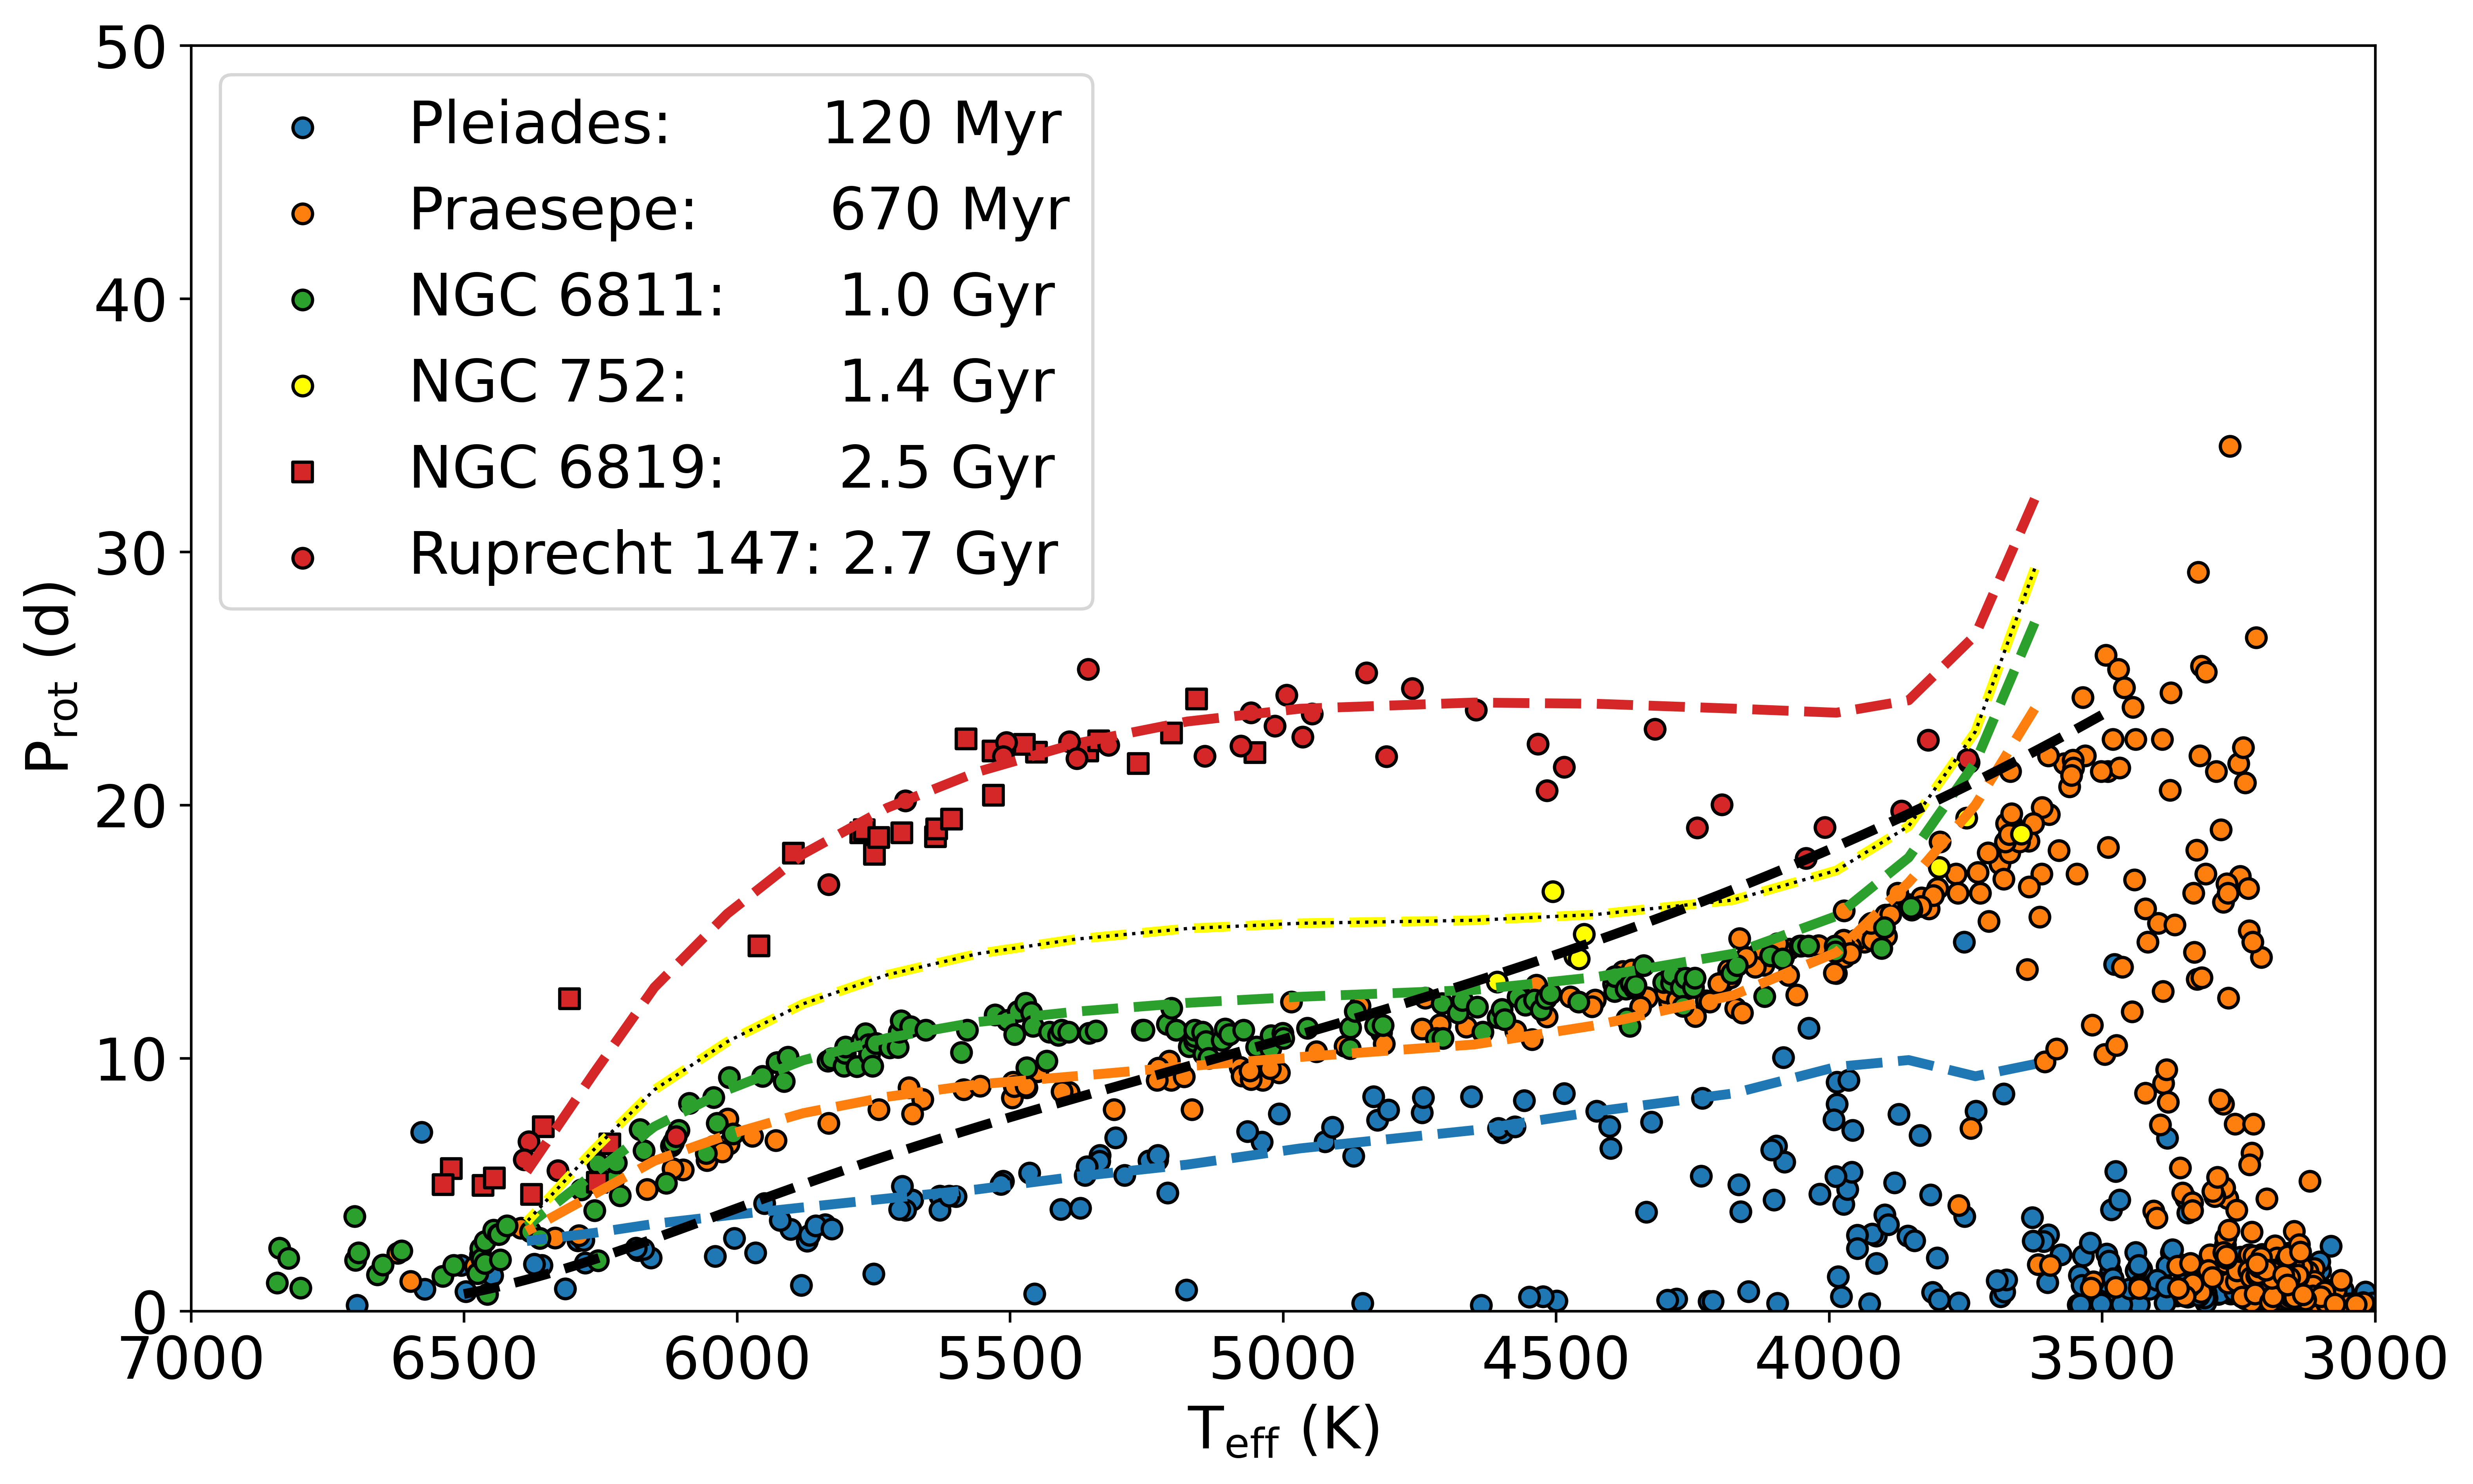
\includegraphics[width=\textwidth]{Figures/rot_gap_figures/com_gap_clus.png}
  \caption[Scatter plot of various cluster rotational periods distributions against effective temperature overlayed on the \kepler{} \citet{mcquillan_rotation_2014} rotational period sample.]{Scatter plot of cluster rotational periods distributions (Pleiades (120 Myr), Praesepe (700 Myr) and NGC 6811 (1 Gyr)) used to tune the rotational isochrones adopted in this work \citep{spada_competing_2020} against effective temperature overlayed on the \kepler{} \citet{mcquillan_rotation_2014} rotational period sample. We have also shown the line $R_o \ = \ 0.45$ in black highlighting that the high temperature ($\>$5000K) Pleiades and Praesepe members may have significant latitudinal differential rotation, biasing the observed rotational periods.}
  \label{fig:com_gap_clus}
\end{figure}

The Sun is believed to be currently transitioning from solar-like to anti-solar-like differential rotation.
As a result of this transition, the average observed, rotation period will decrease suddenly.
We believe this is a feature of the measurement of the average rotation period with differential rotation.
In this work, we have identified the overdensity of stars with solar $R_o$ and the shape of the upper left edge of the rotational period distribution.
While the observed \kepler{} rotation periods do contain a high density of stars near this location (the long-period pileup \citep{van_saders_forward_2019} ), we are hesitant to suggest whether this feature is the result of this transition or from the selection function of \kepler{} observations being biased towards higher mass, brighter, stars.
Further, given the small number of nearby, old ($\geq$ 3 Gyr) clusters in the \kepler{} field, and the evolution of rotational spin-down with variations to the latitudinal differential rotation, we believe that the cluster-tuned isochrones used in this work to determine the rotational periods of stars are less reliable for these stars.
 
 
We believe that this representative study of the effect of differential rotation on the observed rotation periods of stars is a promising avenue to explain the gap.
Further works to confirm this mechanism with more rigorous methods.
We propose the following investigations:
\begin{itemize}
	\item Observations of the differential rotation of nearby stars with Doppler imaging above and below the rotational period gap to search for evidence of variance to latitudinal differential rotation.
	\item Use of more rigorous models of the latitudinal expression of stellar spots and their effect on the observed rotation period of stars. Such an analysis could first be completed with non-uniform distributions of stellar spots on the surface of stars from magnetohydrodynamic simulations of rotating stars using a similar analysis to that performed in this work. We also propose a hare and hound investigation where lightcurves of a synthetic sample of stars with model-motivated stellar spot distributions and observationally motivated differential rotation profiles are then treated as data to determine whether the rotational period gap is recovered using methods of rotational period measurement.
	\item Finally, we propose further modelling work to determine the evolution of surface differential rotation of fully convective stars. If surface differential rotation is suppressed or otherwise peculiar from partially convective stars, then this mechanism can fully explain the observations of \citet{lu_bridging_2022}.
\end{itemize}

\section{Conclusions}
\label{sec:conclusion}

In this work we have qualitatively shown that the transition from latitudinally-flat to equator-fast differential rotation can introduce a dearth of observations in a rotational period distribution.
The transition from latitudinally-flat to equator-fast differential rotation occurs precisely at at $R_o \ = \ 0.45$ coincident with the intermediate period gap.
This suggests that the cause of the intermediate period gap is said transition.
We argue that the growth latitudinal shear explains a number of features of the intermediate period gap, including the high density of stars above and below the gap, and the decrease in photometric variability of stars within the gap.
The scale of the introduced dearth is dependent on highly uncertain parameters that may be degenerate: the latitudinal distribution of stellar spots and the relationship between $R_o$ and latitudinal shear.
These results provide a novel explanation for the intermediate period gap without the requirement of new physics and underscores the need for further research into the impact of latitudinal differential rotation on observations of surface rotation of stars across the main-sequence.

%\appendix*{Observed rotation periods when 1D model rotation period is the average surface rotation period}
%\label{sec:appendix}
%
%If we assume that the output rotation period of the \citet{spada_competing_2020} rotational isochrones is the average rotation period of the surface then we can calculate the equator rotation period and thus the surface rotation profile.
%Adopt a second-order solar-like differential rotation profile with the rotation rate with latitude
%\begin{equation}
%    \Omega\left(\theta\right) = \Omega_{\rm{eq}} - \frac{\Delta \Omega}{\sin^2{60^{\circ}}} \sin^2{\theta}
%\end{equation}
%where \Omega_{\rm{eq}} is the equator rotation rate and $\theta$ is latitude, the average rotation rate on the surface of the star is given by
%\begin{equation}
%	\Omega_{\rm{s,avg}} = \int^{\frac{\pi}{2}}_{0} \Omega(\theta) \sin(\theta) \rm{d}\theta \ / \  \int^{\frac{pi}{2}}_{0} \sin(\theta) \rm{d}\theta = \Omega_{\rm{eq}} - \frac{2}{3}\frac{\Delta \Omega}{\sin^2{60^{\circ}}}
%\end{equation}
%where \Omega_{\rm{s,avg}} is the average rotation rate of the surface, and the equator rotation rate can then be calculated
%\begin{equation}
%	\Omega_{\rm{eq}} = \Omega_{\rm{s,avg}} + \frac{2}{3}\frac{\Delta \Omega}{\sin^2{60^{\circ}}}
%\end{equation}
%Then
%\begin{equation}
%    \label{eq:obs_avg}
%    \Omega_{\rm{prof,avg}}\left(\theta\right) = \Omega_{\rm{s,avg}} + \frac{\Delta \Omega}{\sin^2{60^{\circ}}} \left( \frac{2}{3} - \sin^2{\theta}\right).
%\end{equation}
%The average rotation period corresponds to the rotation period at $\theta \ = \ \sin^{-1}\sqrt{\frac{2}{3}} \sim 55^{\circ}$.
%Therefore $\Omega\left( \theta \right) > \Omega_{\rm{s,avg}}$ while $\theta< 55^{\circ}$ and, after integrating to obtain the observed rotation rate ($\Omega_{\rm{obs,avg}}$) following Equation \ref{eq:inte}, $\Omega_{\rm{obs,avg}} > \Omega_{\rm{s,avg}}$ if the stellar spots are uniformly distributed between $0^{\circ}$ and $60^{\circ}$.
%If we take the ratio of the differences between Equations \ref{eq:obs_avg}and \ref{eq:obs_eq} and the model rotation rate ($\Omega_{s,avg}$ and $\Omega_{\eq}$), which to be clear are equal but are differentiated for clarity,
%\begin{equation}
%	\frac{\Omega_{\rm{s,avg}} - \int^{\theta_{\rm{max}}}_{\theta_{\rm{min}}} \left( \Omega_{\rm{s,avg}} + \frac{\Delta \Omega}{\sin^2{60^{\circ}}} \left( \frac{2}{3} - \sin^2{\theta}\right)  \right )\sin(\theta) \rm{d}\theta}{\Omega_{\rm{eq}} - \int^{\theta_{\rm{max}}}_{\theta_{\rm{min}}} \left( \Omega_{\rm{eq}} - \frac{\Delta \Omega}{\sin^2{60^{\circ}}} \sin^2{\theta} \right )\sin(\theta) \rm{d}\theta} = \frac{\Omega_{s,avg} - \Omega_{\rm{obs,avg}}}{\Omega_{eq} - \Omega_{\rm{obs,eq}}}
%\end{equation}
%where $\Omega_{\rm{obs,eq}$ is the observed rotation rate assuming the injected rotation rate is the equator rotation rate, then as $\Omega_{\rm{obs,avg}} > \Omega_{\rm{s,avg}}$ and $\Omega_{\rm{obs,avg}} > \Omega_{\rm{obs,eq}}$, it is clear that  the introduced variation to the observed rotation period compared to the injected rotation period ($P_{\rm{s,avg}}$ and $P_{\rm{eq}}$) is smaller if we take the injected rotation period as the average rotation period of the surface.
%
%To show this more clearly, in Figure \ref{fig:}, we show effect of this assumption on the observed rotation period against injected rotation period of a 0.7 $M_{\odot}$ star with a uniform distribution of stellar spots between $0^{\circ}$ and 60$^{\circ}$.
%Comparing this Figure to Figure \ref{fig:} it is clear that the introduction of equator fast latitudinal differential rotation decreases the observed rotation period and that the scale of the difference between the injected and observed rotation periods is smaller under this assumption.




